\documentclass[a4paper,12pt]{article}
\usepackage[utf8]{vietnam}
\usepackage{hyperref}
\usepackage{graphicx}
\usepackage{xcolor}
\usepackage{subfigure}
\usepackage{float}
\usepackage{caption}
\hypersetup{
	pdfborder = {0 0 0}
}
\title{\textbf{Báo cáo tuần 6 \\ Thực hành kiến trúc máy tính}}
\author{Họ tên: Phan Minh Anh Tuấn \\ MSSV: 20205227}
\date{}
\begin{document}
	\maketitle
	\tableofcontents
	\newpage
\section{Assignment 1}
\begin{figure}[!h]
	\centerline{\fbox{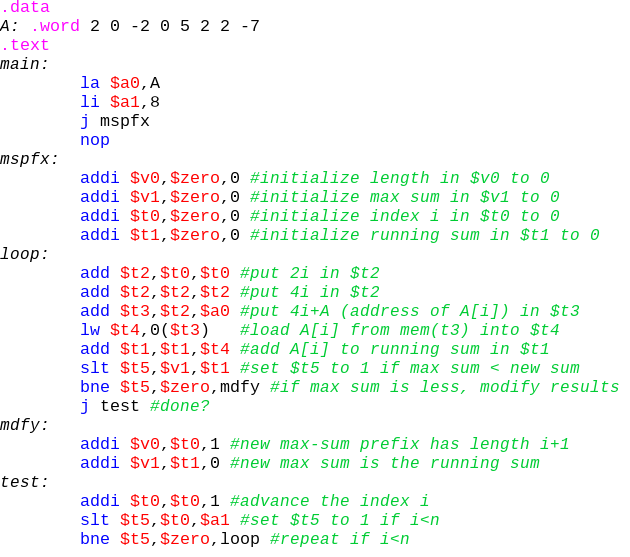
\includegraphics[width=0.7\textwidth]{ass1/code.png}}}
	\caption{Code của Assignment 1}
	\label{fig:ass1}
\end{figure}
\noindent
\textbf{Trong đó: }
\begin{itemize}
	\item \$a0 lưu địa chỉ phần tử đầu của mảng A
	\item \$a1 lưu số phần tử của mảng A
	\item mspfx là chương trình khởi tạo các biến độ dài mảng, tổng lớn nhất, index và tổng hiện thời
	\item loop là vòng lặp thực hiện để tính tổng
	\item mdfy là chương trình cập nhật tổng lớn nhất
	\item test là chương trình kiểm tra điều kiện lặp
\end{itemize}
\textbf{Giải thích thuật toán: }Đi từ đầu đến cuối mảng, nếu max sum (\$v1) < running sum (\$t1) thì cập nhật max sum = running sum, nếu không vẫn giữ nguyên.
\clearpage
\section{Assignment 2}
\begin{figure}[!h]
	\centering
	\subfigure{ 
		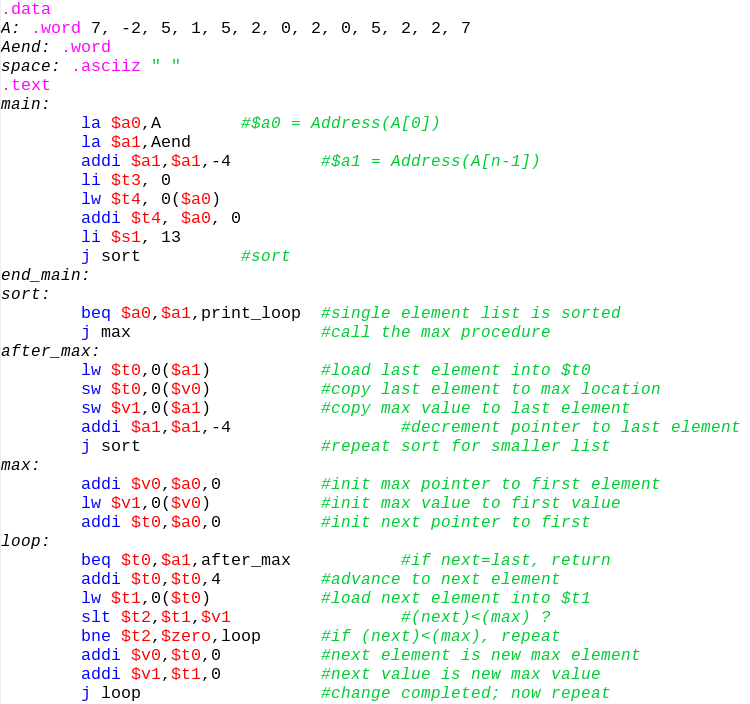
\includegraphics[scale = 0.4]{ass2/code1.png}
		\label{Mạch 2}} 
	\subfigure{ 
		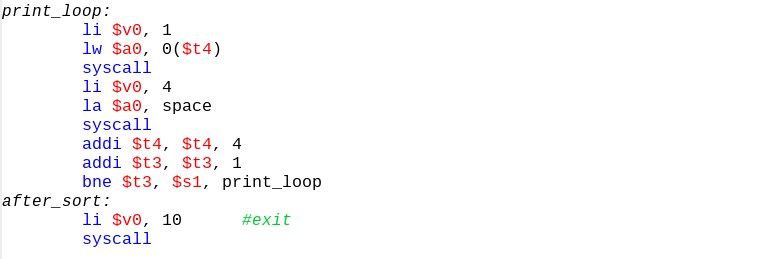
\includegraphics[scale = 0.4]{ass2/code2.png}
		\label{Mạch 1}} 
	\caption{Code của Assignment 2} 
\end{figure}
\noindent
\textbf{Giải thích thuật toán Selection Sort: }Bắt đầu bằng việc chọn vị trí đầu làm mốc, đi từ đầu đến cuối mảng (trừ vị trí mốc) duyệt tìm phần tử bé nhất. Sau khi duyệt xong đổi chỗ phần tử bé nhất và phần tử tại vị trí mốc, lúc này vị trí mốc đã được xếp đúng vị trí. Tiếp tục với các phần tử vị trí cao hơn.
\clearpage
\begin{figure}[!h]
	\centerline{\fbox{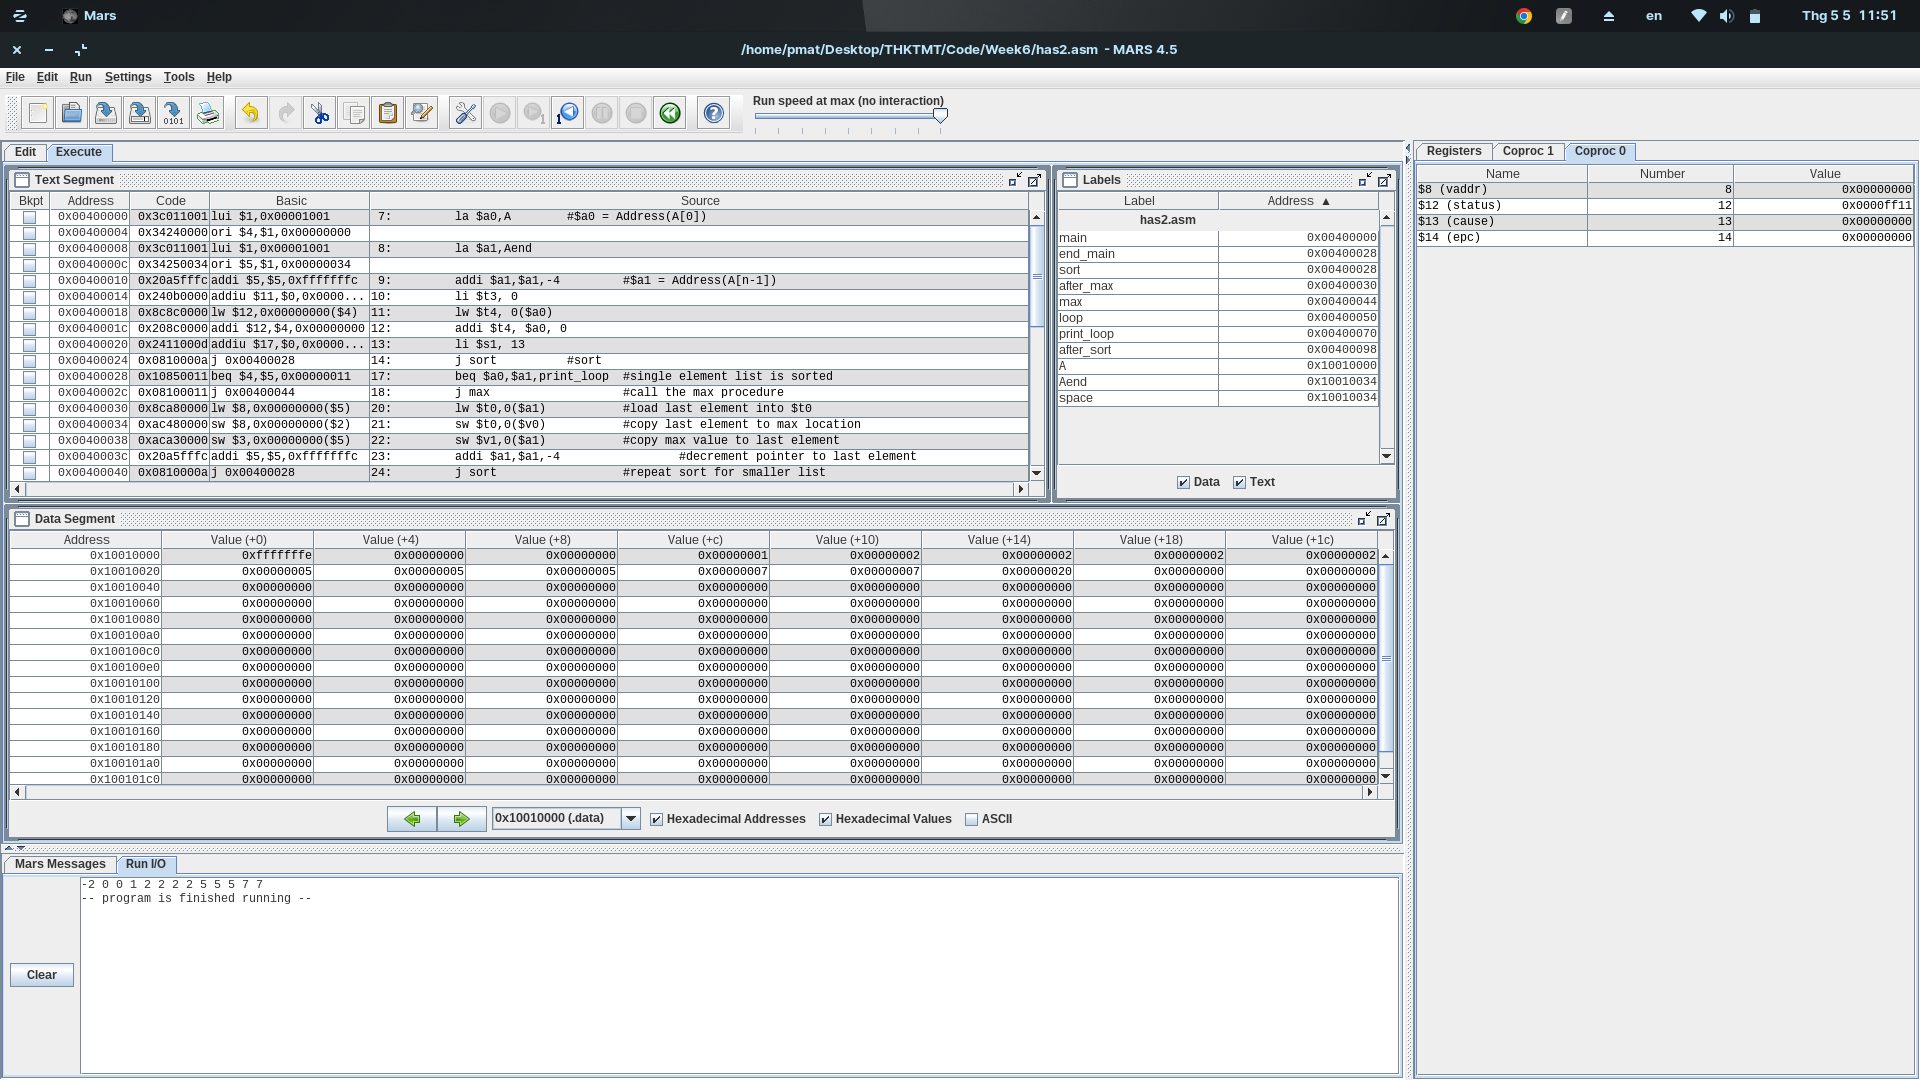
\includegraphics[width=1\textwidth]{ass2/kq.png}}}
	\caption{Kết quả của Assignment 2}
	\label{fig:ass2}
\end{figure}
\noindent
Mảng đầu vào: 7, -2, 5, 1, 5, 2, 0, 2, 0, 5, 2, 2, 7 \\
Mảng sau khi đã sắp xếp: -2, 0, 0, 1, 2, 2, 2, 2, 5, 5, 5, 7, 7 
\clearpage
\section{Assignment 3}
\begin{figure}[!h]
	\centering
	\subfigure{ 
		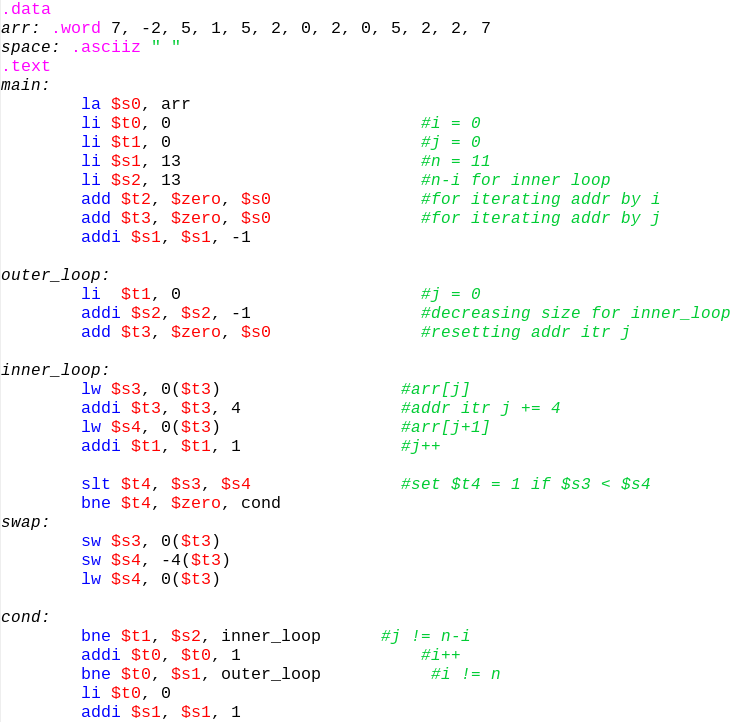
\includegraphics[scale = 0.4]{ass3/code1.png}
		\label{Mạch 3}} 
	\subfigure{ 
		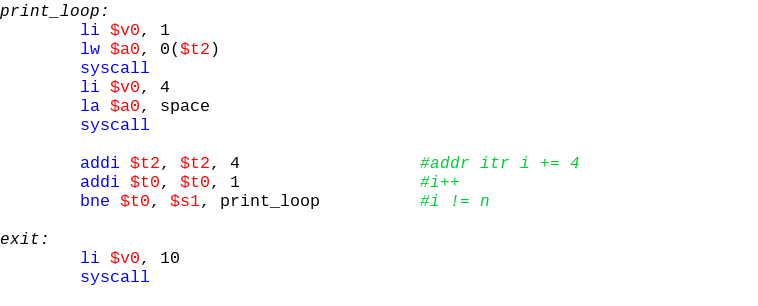
\includegraphics[scale = 0.4]{ass3/code2.png}
		\label{Mạch 4}} 
	\caption{Code của Assignment 3} 
\end{figure}
\noindent
\textbf{Giải thích thuật toán Bubble Sort: } Đi từ đầu đến cuối mảng so sánh hai phần tử kề nhau, nếu chúng chưa đứng đúng thứ tự thì đổi chỗ (swap). Có thể tiến hành từ trên xuống (bên trái sang) hoặc từ dưới lên
\clearpage
\begin{figure}[!h]
	\centerline{\fbox{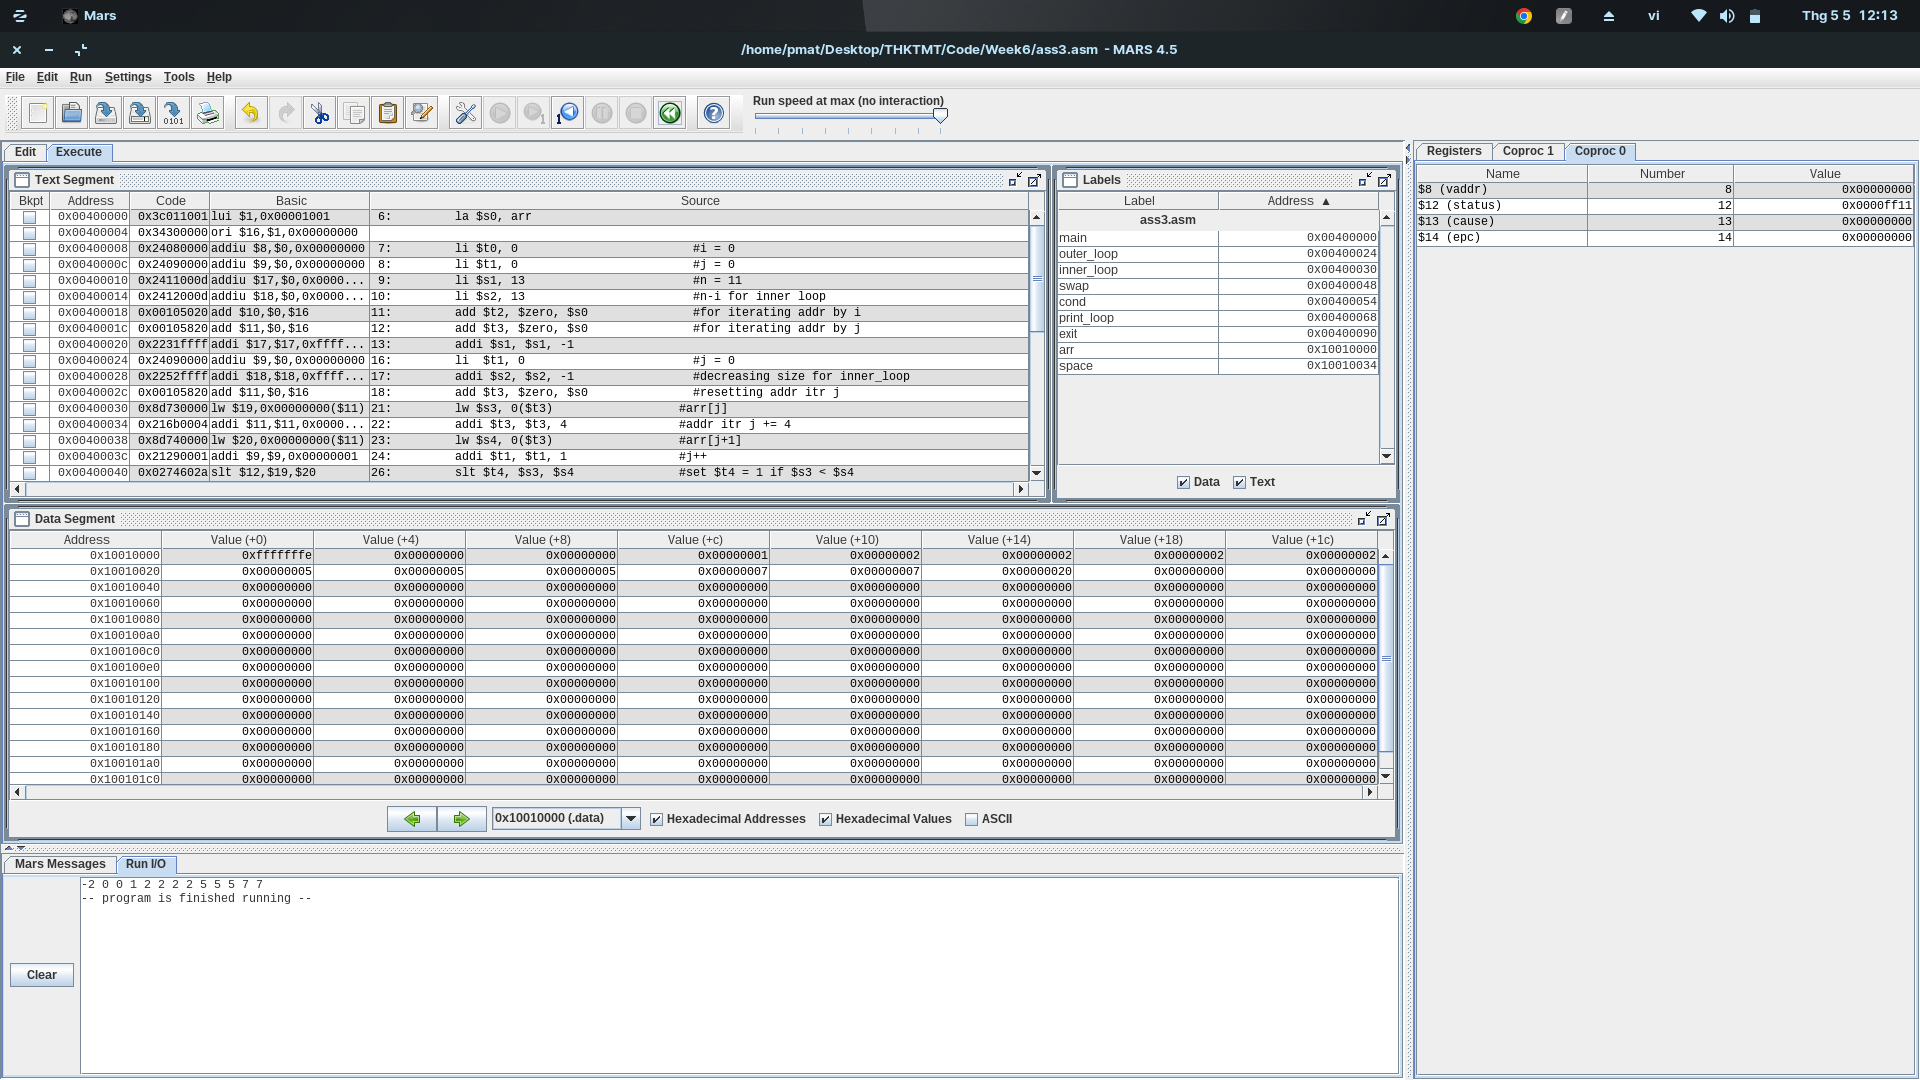
\includegraphics[width=1\textwidth]{ass3/kq.png}}}
	\caption{Kết quả của Assignment 3}
	\label{fig:ass3}
\end{figure}
\noindent
Mảng đầu vào: 7, -2, 5, 1, 5, 2, 0, 2, 0, 5, 2, 2, 7 \\
Mảng sau khi đã sắp xếp: -2, 0, 0, 1, 2, 2, 2, 2, 5, 5, 5, 7, 7 
\clearpage
\section{Assignment 4}
\begin{figure}[!h]
	\centering
	\subfigure{ 
		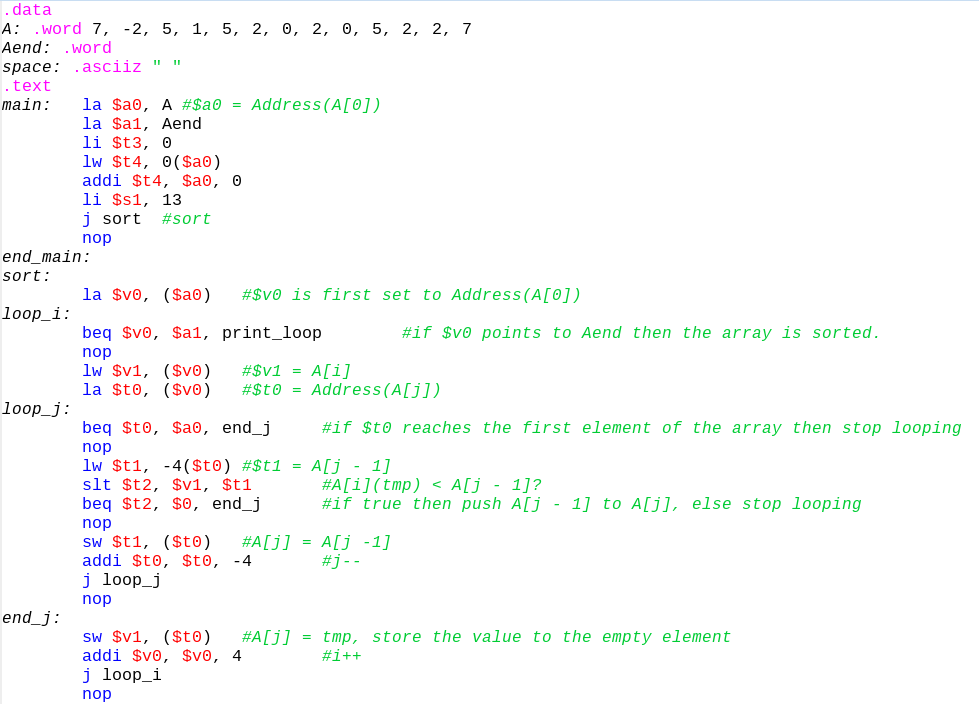
\includegraphics[scale = 0.4]{ass4/code1.png}
		\label{Mạch 5}} 
	\subfigure{ 
		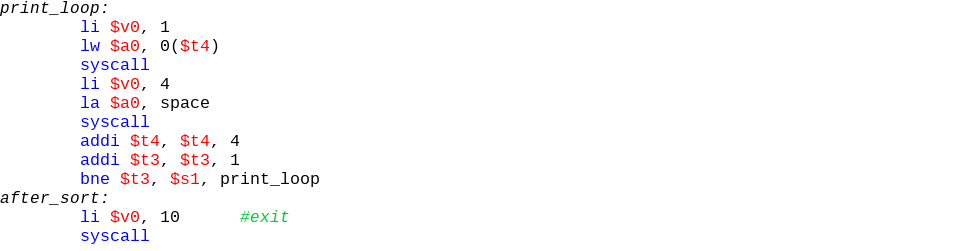
\includegraphics[scale = 0.4]{ass4/code2.png}
		\label{Mạch 6}} 
	\caption{Code của Assignment 4} 
\end{figure}
\noindent
\textbf{Giải thích thuật toán Insertion Sort: } muốn sắp mảng theo trật tự, ta bắt đầu từ phần tử thứ 2, so với các phần tử đứng trước nó để chèn vào vị trí thích hợp.
\clearpage
\begin{figure}[!h]
	\centerline{\fbox{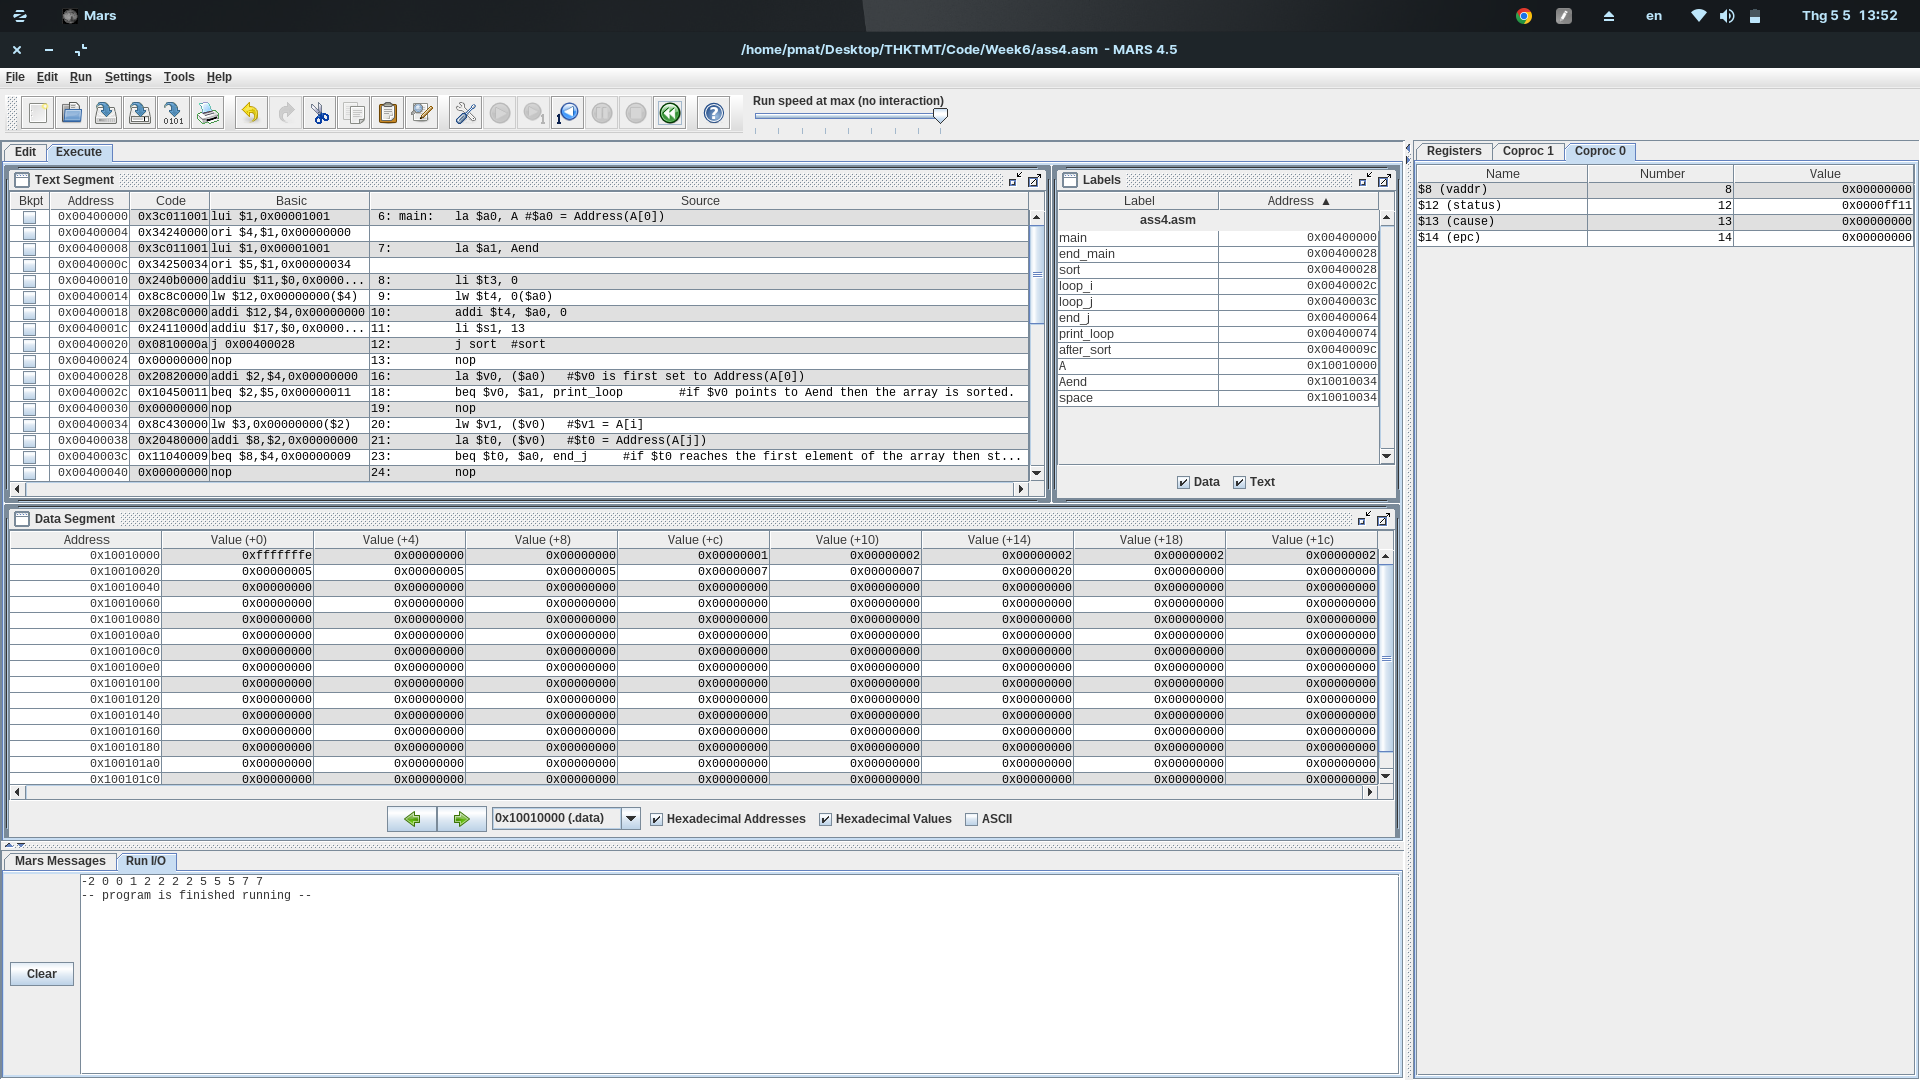
\includegraphics[width=1\textwidth]{ass4/kq.png}}}
	\caption{Kết quả của Assignment 4}
	\label{fig:ass4}
\end{figure}
\noindent
Mảng đầu vào: 7, -2, 5, 1, 5, 2, 0, 2, 0, 5, 2, 2, 7 \\
Mảng sau khi đã sắp xếp: -2, 0, 0, 1, 2, 2, 2, 2, 5, 5, 5, 7, 7 
\end{document}